\chapter{Апробация решения} \label{ch4}

\section{Оценка ExCodeAgent-MM} \label{ch4:sec1}

``Ядром'' предлагаемого решения ExCodeAct является агент кодогенерации ExCodeAgent-MM:
именно он в апробации использует бо'льшую часть спектра предлагаемых инструментов. 

Ввиду специфики задачи (а именно создание MAS для работы \textit{с внутренними} 
инструментами), использование публичных бенчмарков для тестирования является в определенном
смысле нецелесообразным и бессмысленным: важно оценить качество агента именно в применении внутренних
инструментов, информация о которых была или недоступной или малоизвестной для LLM-моделей.

Потому ниже будет представлено полное изложение анализа предлагаемого решения и сравнения
его с аналогами в кодогенерации с использованием внешних источников.

\subsection{ClearML-bench - бенчмарк для оценки работы с окружением посредством кодогенерации} \label{ch4:sec1:subsec1}

В рамках тестирования корректности работы агента кодогенерации был создан собственный  
бенчмарк ClearML-bench, содержащий 15 вопросов-сценариев для оценки корректности взаимодействия 
с окружением в различных вариациях: работа с датасетами (создание, загрузка и выгрузка), 
работа с данными (преобразования, визуализации, анализ и сохранение), обучение моделей.

Сами задачи разбиты на 7 простых атомарных задач, требующие работу с малой частью функционала одного
инструмента, и на 8 комплексных задач, представляющих различные \textit{реальные} сценарии использования
агента: от анализа работы нейросетей с разными видами предобработки данных до полного цикла
обучения сети на облачных данных с последующей валидацией на других, также облачных данных.

Принцип, по которому происходит тестирование, описывается просто: каждое задание направлено на 
определенный набор взаимодействий с окружением (будь оно или локальной файловой
системой, или системой ClearML, или и тем и другим вместе). 
Сначала, перед запуском агента кодогенерации, производится оценка окружения - 
так формируется начальное, $t_0$ описание окружения. 
Описание окружения состоит из описания содержимого ожидаемой рабочей директорией агента, 
с которой предполагается работа (файлы, директории), а также из описания содержимого самого ClearML: какие
датасеты и задания на текущий момент там находятся. После этого производится запуск
агента кодогенерации с определенным текстовым заданием с последующим снятием 
конечного описания окружения $t_1$. Поскольку все представленные выше элементы 
описания окружения можно представить в виде множеств, над которым определена операция разности, 
можно посчитать разность $\delta t = t_1 \backslash t_0$ и сравнить её с тем,
какой результат ожидался. В случае совпадения ожидания задание засчитывается и ставится 1 балл, 
иначе - 0 баллов.

Хоть бенчмарк и назван в честь инструмента менеджмента данных и моделей ClearML, 
тестирование охватывает сценарии с применением \textit{различных} инструментов: 
ClearML носит больше описательную характеристику окружения, 
с которым инструменты отчасти иногда взаимодействуют.

Полное и развернутое описание содержимого бенчмарка представлено в Приложении №\ref{appendix-clearml-bench}. 

\subsection{Используемые инструменты} \label{ch4:sec1:subsec2}
В ходе тестирования принимало участие
5 внутренних кодовых инструмента:
\begin{itemize}
    \item ``cloudml\_manager'' - модификация Python SDK ClearML для 
автоматического структурирования артефактов деятельности лаборатории (датасетов, заданий, 
моделей) по проектам;
    \item ``deconvolution\_module'' - модуль с классами и статическими методами 
для работы с трехмерными изображениями и их улучшения при помощи нейросетевого алгоритма деконволюции;
    \item ``denoising\_module'' - модуль с классом и статическими методами 
для работы с трехмерными изображениями и их улучшения при помощи нейросетевого алгоритма денойзинга;
    \item ``biobert\_module'' - модуль с классом и статическими методами для
работы с сигналами активности мозга; использовался как дополнительный функционал в рамках
тестирования для оценки длины контекста и качества выбора нужного инструмента;
    \item ``spinetool\_module'' - модуль с классом и статическими мокап (mockup) методами для
работы с трехмерными моделями дендритных шипов; использовался как дополнительный 
функционал в рамках тестирования для оценки длины контекста и 
качества выбора нужного инструмента. 
\end{itemize}

Полный список используемых инструментов лаборатории, а также то, как они описывались для LLM-агентов, 
представлен в Приложении №\ref{appendix-tools}.

\subsection{Сравнение конфигураций ретриверов} \label{ch4:sec1:subsec3}

Тестирование ExCodeAgent-MM производилось как на различных способах подачи информации о кодовых инструментах В
контекст, так и на различных размерах модели. В данном подпараграфе описывается первое исследование.

В сравнении вариантов добавления документации в контекст принимало участие 4 вариации:
\begin{itemize}
	\item Coarse-Fine RAG - предлагаемая разработка интеграции документации в контекст;
	\item All in SP (system-prompt) - передача всей документации единым блоком в системном промпте;
	\item Common RAG (recursive) - классическая вариация RAG на основе косинусного сходства вопроса и частей
документации, разбитого при помощи рекурсивного разбиения документов;
	\item Common RAG (semantic) - классическая вариация RAG на основе косинусного сходства вопроса и частей
документации, разбитого семантически на блоки, отвечающих описанию конкретного метода или класса.
\end{itemize}

В качестве LLM-модели использовался Codestral-latest - большой языковой модели Mistral, специализирующейся
на выполнения задач, связанных с кодом. Семейство моделей Mistral доступна по API.

В качестве измеряемых параметров, помимо числа баллов в бенчмарке ClearML-bench, были
еще время работы и количество использованных токенов.

\begin{figure}
    \center
	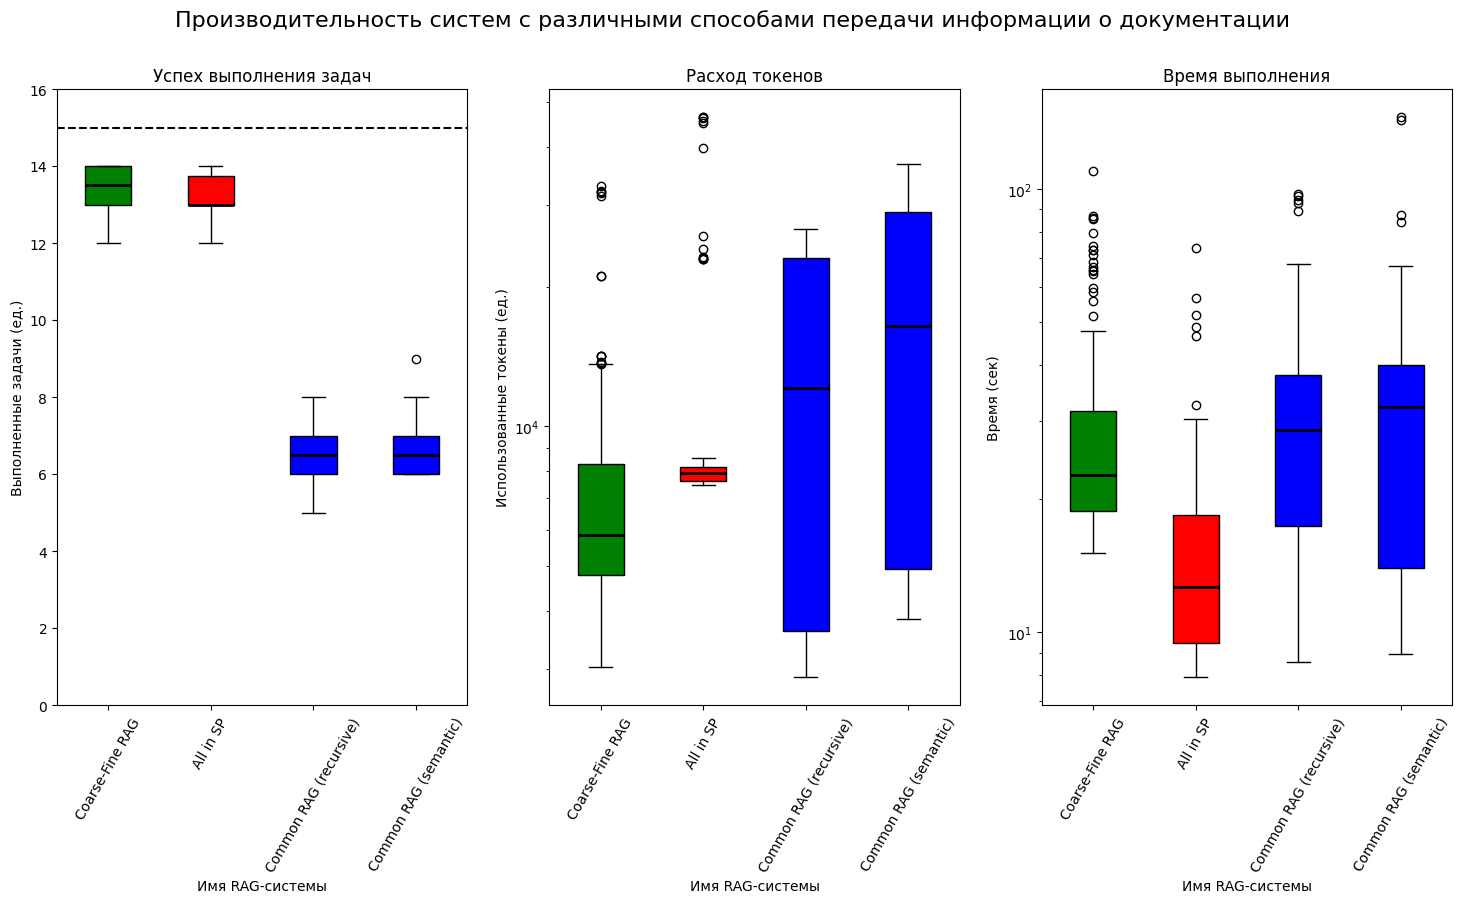
\includegraphics[scale=0.42]{sources/stats_1.png}
	\caption{Результаты работы ExCodeAgent-MM на различных ретриверах.} 
	\label{fig:ch4:rags}  
\end{figure}

\begin{table}[t!]% Пример оформления таблицы
	\centering\small
	\caption{Значения выборочных средних и СКО для каждого параметра и конфигурации агента. 
Жирным выделены лучшие значения оценок среди различных конфигураций. У остальных значений
в строках дополнительно указаны в скобках процентные отклонения от лучшего значения.}%
	\label{tab:ch4:values}		
	\begin{tabular}{|l|l|l|l|l|l|}
		\hline
		Values&Coarse-fine RAG&All in SP&RAG (recursive)&RAG (semantic)\\
		\hline
		$\mu_{tasks}$ (ед.)&\textbf{13.4}&13.1 $(-2,2\%)$&6.4 $(-52,2\%)$&6.8 $(-49,2\%)$\\ \hline
		$\sigma_{tasks}$ (ед.)&\textbf{0.7}&0.74 $(+5,7\%)$&0.97 $(+38,6\%)$&1. $(+42,9\%)$\\ \hline
		$\mu_{tokens}$ (ед.)&\textbf{7812.7}&10162.2 $(+30,1\%)$&14073.3 $(+80,2\%)$&17817.4 $(+128,1\%)$\\ \hline
		$\sigma_{tokens}$ (ед.)&\textbf{5543}&7991 $(+44,2\%)$&8503 $(+53,4\%)$&10988 $(+98,2\%)$\\ \hline
		$\mu_{times}$ (сек.)&30.2 $(+91,2\%)$&\textbf{15.8}&30. $(+89,9\%)$&31.6 $(+100\%)$\\ \hline
		$\sigma_{times}$ (сек.)&18 $(+87,5\%)$&\textbf{9.6}&17.3 $(+80,2\%)$&20.9 $(+117,7\%)$\\ \hline		
	\end{tabular}	
	\normalsize% возвращаем шрифт к нормальному
\end{table}


На \firef{fig:ch4:rags} представлены результаты работы ExCodeAgent-MM на различных 
ретриверах. Значение оценки среднего положения и несмещенной оценки среднеквадратичного отклонения
представлены в таблице \ref{tab:ch4:values}.

Из графиков и табличных значений видно, что качество выполнения задач в первых двух ретриверах практически 
одинаково: практически одинаковы выборочные среднее и дисперсия. Однако стоит отметить, что количество 
используемых токенов при генерации решений у второго ретривера в 1.5 раза больше - и это только на конкретном
небольшом наборе инструментов: ввиду того, что метод подачи всей документации в один контекст модели плохо
масштабируется с ростом числа кодовых инструментов, данный показатель в 1.5 процента не является пределом.
Важно отметить тот факт, что стандартные ретриверы, как и ожидалось, должного качества не обеспечивают - связано
это как с отсутствием учета семантического содержимого, так и с отсутствием учета структуризированности 
документаций. 

Стоит и выделить и неприятное наблюдение: предлагаемое решение требует в два раза больше времени для решения
одной задачи - это обуславливается дополнительными двумя запросами для LLM-моделей. Стоит отметить, что ввиду
``плохого качества'' решений стандартных ретриверов при первых генерациях, данное замедление наблюдается и 
у других методов селекции релевантного контекста документаций. 

\subsection{Сравнение различных размеров моделей} \label{ch4:sec1:subsec4}

Для оценки работоспособности агента ExCodeAgent-MM в зависимости от выбора размеров большой языковой
модели было проведено дополнительное тестирование со следующими LLM-моделями:
\begin{itemize}
    \item Codetral-latest - большая модель семейства Mistral, специализированная по работе с кодом;
    \item Mistral-Large-instruct - большая модель семейства Mistral общего назначения;
    \item Mistral-Small-instruct - маленькая модель семейства Mistral на 8B параметров;
    \item Mistral-Mini-instruct - самая маленькая модель семейства Mistral на 3B параметров;
\end{itemize} 
Все данные модели были запущены на удаленных вычислительных мощностях, предоставляемые
самим Mistral по API. В качестве ретривера использовался Coarse-Fine RAG.

\begin{figure}
    \center
	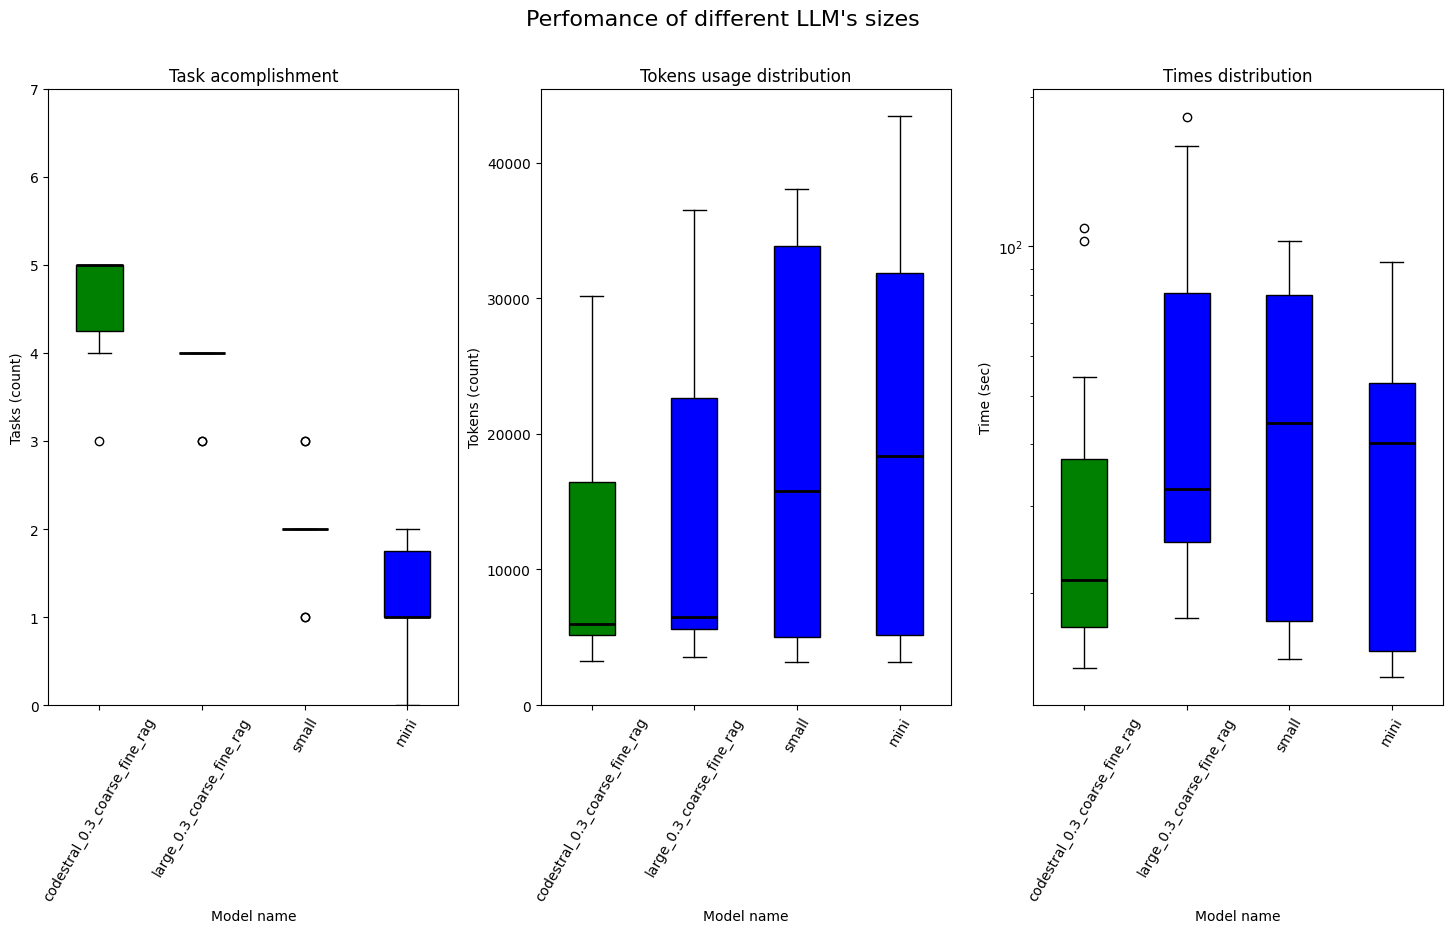
\includegraphics[scale=0.42]{sources/stats_2.png}
	\caption{Результаты работы ExCodeAgent-MM на различных моделях.} 
	\label{fig:ch4:llms}  
\end{figure}

\begin{table}[t!]% Пример оформления таблицы
	\centering\small
	\caption{Значения выборочных средних и СКО для каждого параметра и LLM-модели. 
Жирным выделены лучшие значения оценок среди различных конфигураций. У остальных значений
в строках дополнительно указаны в скобках процентные отклонения от лучшего значения.}%
	\label{tab:ch4:values}		
	\begin{tabular}{|l|l|l|l|l|l|}
		\hline
		Values&Codestral&Mistral-Large&Mistral-Small&Mistral-Mini\\
		\hline
		$\mu_{tasks}$ (ед.)&\textbf{13.4}&12.4 $(-7,4\%)$&5.1 $(-61,9\%)$&2.4 $(-82\%)$\\ \hline
		$\sigma_{tasks}$ (ед.)&\textbf{0.7}&0.7 $(0\%)$&0.86 $(+22\%)$&0.7 $(0\%)$\\ \hline
		$\mu_{tokens}$ (ед.)&\textbf{7812.7}&9931 $(+27\%)$&15101 $(+93\%)$&16303 $(+108,6\%)$\\ \hline
		$\sigma_{tokens}$ (ед.)&\textbf{5543}&8408 $(+51,6\%)$&14342 $(+158,7\%)$&11908 $(+114,8\%)$\\ \hline
		$\mu_{times}$ (сек.)&\textbf{30.2}&41.7 $(+38\%)$&45.9 $(+52\%)$&37 $(+22,5\%)$\\ \hline
		$\sigma_{times}$ (сек.)&\textbf{18}&23.4 $(+30\%)$&30.3 $(+68,3\%)$&20 $(+11,1\%)$\\ \hline		
	\end{tabular}	
	\normalsize% возвращаем шрифт к нормальному
\end{table}

На рисунке \firef{fig:ch4:llms} представлены результаты работы ExCodeAgent-MM на 
различных больших языковых моделях. Из графико видно, что как 
специализированная, так и обычная большая модель общего назначения, практически одинаково 
хорошо решают задачи из бенчмарка: единственная разница заключается в количестве
попыток генерации кода для решении задач - у модели общего назначения их больше. 
Однако, малые модели плохо справляются с решением задач.

% \begin{figure}
%     \center
% 	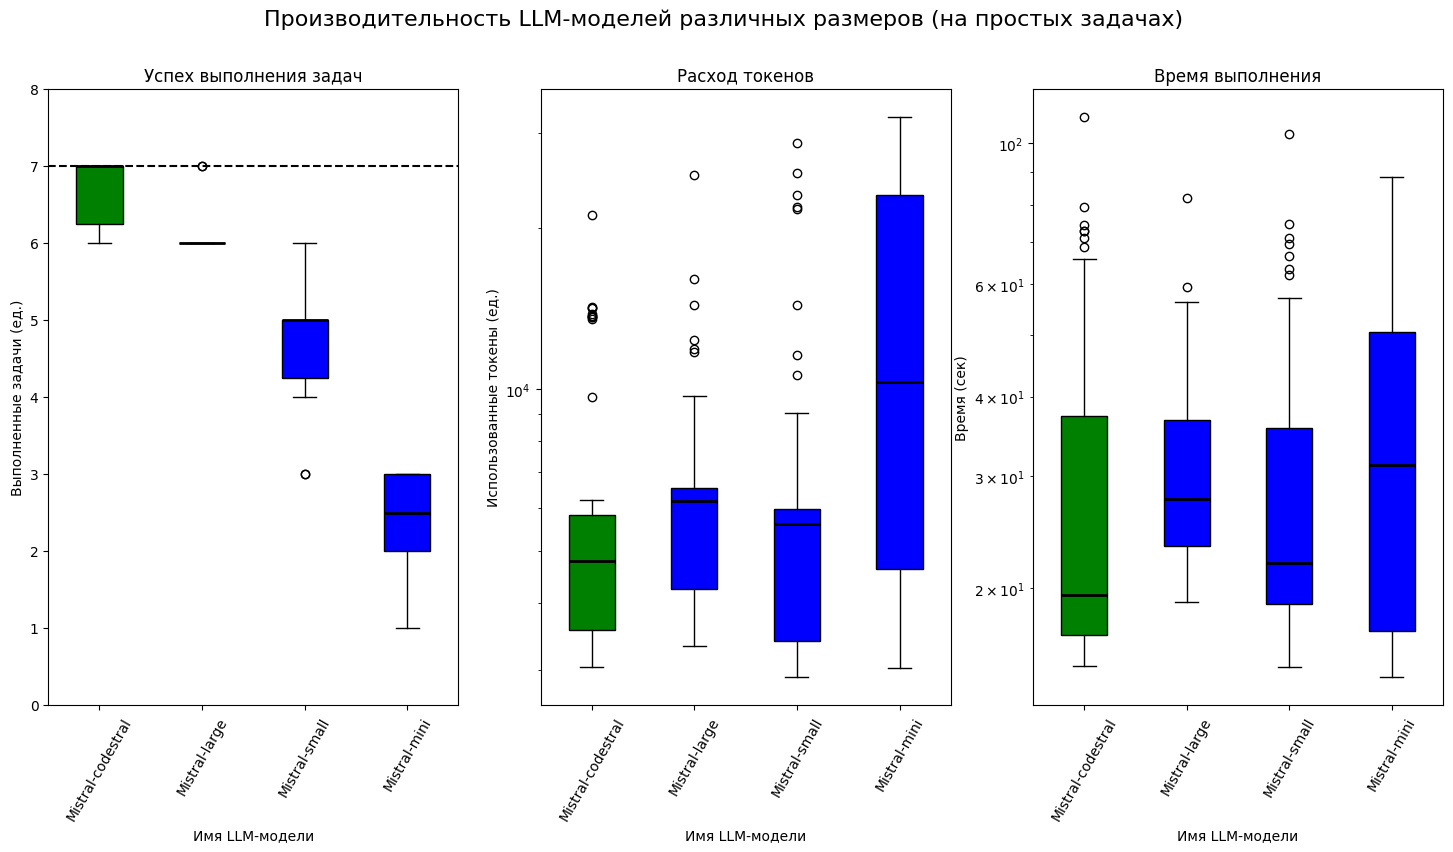
\includegraphics[scale=0.42]{sources/stats_21.png}
% 	\caption{Результаты работы ExCodeAgent-MM на различных моделях (на простых задачах).} 
% 	\label{fig:ch4:llms_easy}  
% \end{figure}

% \begin{figure}
%     \center
% 	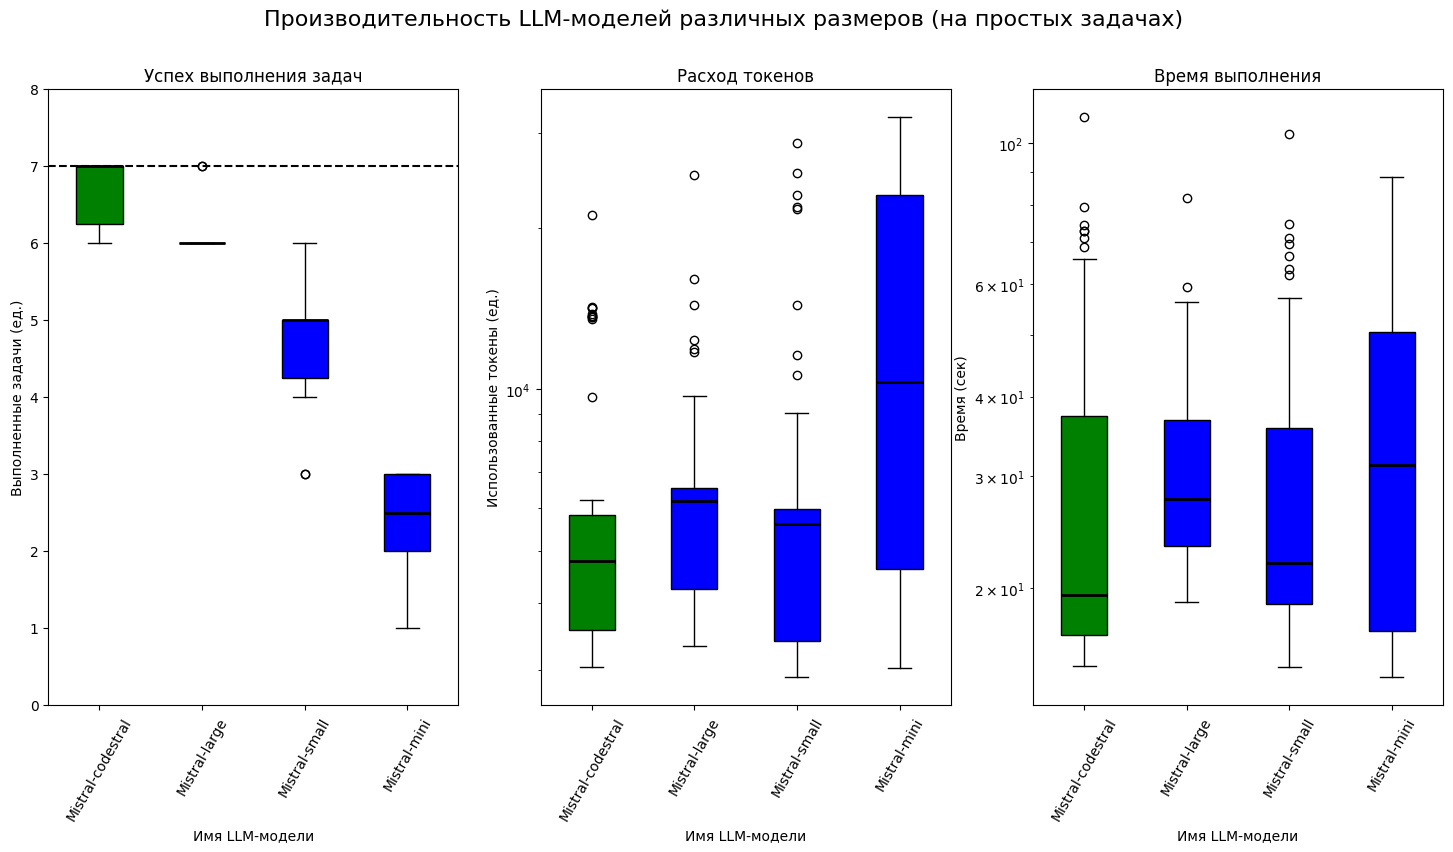
\includegraphics[scale=0.42]{sources/stats_21.png}
% 	\caption{Результаты работы ExCodeAgent-MM на различных моделях (на комплексных задачах).} 
% 	\label{fig:ch4:llms_hard}  
% \end{figure}
% . Однако,
% если обратиться к графикам \firef{fig:ch4:llms_easy} и \firef{fig:ch4:llms_hard}, мы можем увидеть,
% что малые модели плохо справляются именно с комплексными задачами, 

\subsection{Прочие качественные результаты.} \label{ch4:sec1:subsec5}

В данной секции приведены качественные результаты, которые трудно поддаются измерениям, но которые
необходимо отметить как отдельные выдающиеся свойства разработанной системы.

Среди них, конечно же, автоматическая генерация Jupyter Notebook, содержащие полученные успешные кодогенерации
с результатами исполнения, которые поддаются сохранению в формате вывода (текст, изображения).

Также стоит отметить возможность добавления анализа различных модальностей при помощи моделей Modal-To-Text:
они позволяют в последствии интерпретировать сложные модальности при помощи естественного языка.
В приложении №\ref{appendix-multimodal} представлен пример такого вывода на задаче сравнения снимка до и после
деконволюции: можно отметить, что в данном случае модель представляет дополнительную оценку 
качества деконволюции при сравнении снимков.

Важным свойством является и способность масштабирования наборов инструментов при кодогенерации: наиболее успешная
после Coarse-Fine RAG ретривер-система - ``All in SP''. Именно она и не имеет склонности к масштабирования.